% THIS IS SIGPROC-SP.TEX - VERSION 3.1
% WORKS WITH V3.2SP OF ACM_PROC_ARTICLE-SP.CLS
% APRIL 2009
%
% It is an example file showing how to use the 'acm_proc_article-sp.cls' V3.2SP
% LaTeX2e document class file for Conference Proceedings submissions.
% ----------------------------------------------------------------------------------------------------------------
% This .tex file (and associated .cls V3.2SP) *DOES NOT* produce:
%       1) The Permission Statement
%       2) The Conference (location) Info information
%       3) The Copyright Line with ACM data
%       4) Page numbering
% ---------------------------------------------------------------------------------------------------------------
% It is an example which *does* use the .bib file (from which the .bbl file
% is produced).
% REMEMBER HOWEVER: After having produced the .bbl file,
% and prior to final submission,
% you need to 'insert'  your .bbl file into your source .tex file so as to provide
% ONE 'self-contained' source file.
%
% Questions regarding SIGS should be sent to
% Adrienne Griscti ---> griscti@acm.org
%
% Questions/suggestions regarding the guidelines, .tex and .cls files, etc. to
% Gerald Murray ---> murray@hq.acm.org
%
% For tracking purposes - this is V3.1SP - APRIL 2009

\documentclass{acm_proc_article-sp}
\usepackage{auto-pst-pdf}

\begin{document}

\title{A Protocol to Integrate Invasive Resource Management into Standard Batch Schedulers}
%
% You need the command \numberofauthors to handle the 'placement
% and alignment' of the authors beneath the title.
%
% For aesthetic reasons, we recommend 'three authors at a time'
% i.e. three 'name/affiliation blocks' be placed beneath the title.
%
% NOTE: You are NOT restricted in how many 'rows' of
% "name/affiliations" may appear. We just ask that you restrict
% the number of 'columns' to three.
%
% Because of the available 'opening page real-estate'
% we ask you to refrain from putting more than six authors
% (two rows with three columns) beneath the article title.
% More than six makes the first-page appear very cluttered indeed.
%
% Use the \alignauthor commands to handle the names
% and affiliations for an 'aesthetic maximum' of six authors.
% Add names, affiliations, addresses for
% the seventh etc. author(s) as the argument for the
% \additionalauthors command.
% These 'additional authors' will be output/set for you
% without further effort on your part as the last section in
% the body of your article BEFORE References or any Appendices.

\numberofauthors{3} %  in this sample file, there are a *total*
% of EIGHT authors. SIX appear on the 'first-page' (for formatting
% reasons) and the remaining two appear in the \additionalauthors section.
%
\author{
% You can go ahead and credit any number of authors here,
% e.g. one 'row of three' or two rows (consisting of one row of three
% and a second row of one, two or three).
%
% The command \alignauthor (no curly braces needed) should
% precede each author name, affiliation/snail-mail address and
% e-mail address. Additionally, tag each line of
% affiliation/address with \affaddr, and tag the
% e-mail address with \email.
%
% 1st. author
\alignauthor
Nishanth Nagendra\\
       \affaddr{Technical University of Munich}\\
       \affaddr{Institute for Informatics, I10}\\
       \affaddr{Boltzmannstr.3, D-85748 Garching, Germany}\\
       \email{ga38sok@mytum.de}
% 2nd. author
\alignauthor
M.Sc. Isaias Alberto Compres Urena\\
       \affaddr{Technical University of Munich}\\
       \affaddr{Institute for Informatics, I10}\\
       \affaddr{Boltzmannstr.3, D-85748 Garching, Germany}\\
       \email{compresu@in.tum.de}
% 3rd. author
\alignauthor 
Prof. Dr. Michael Gerndt\\
       \affaddr{Technical University of Munich}\\
       \affaddr{Institute for Informatics, I10}\\
       \affaddr{Boltzmannstr.3, D-85748 Garching, Germany}\\
       \email{gerndt@in.tum.de}
}
% There's nothing stopping you putting the seventh, eighth, etc.
% author on the opening page (as the 'third row') but we ask,
% for aesthetic reasons that you place these 'additional authors'
% in the \additional authors block, viz.

% Just remember to make sure that the TOTAL number of authors
% is the number that will appear on the first page PLUS the
% number that will appear in the \additionalauthors section.

\maketitle
\begin{abstract}
Invasive computing is a novel paradigm for the design and resource-aware programming of future parallel computing systems. It enables the programmer to write resource aware programs and the goal is to optimize the program for the available resources. Traditionally, parallel applications implemented using MPI are executed with a fixed number of MPI processes while submitting to a High Performance Computing(HPC) center. This
results in a fixed allocation of resources for the job. Newer techniques in scientific computing such as Adaptive Mesh Refinement(AMR) result in applications exhibiting complex behavior where their resource requirements change during execution. Invasive MPI which is a part of an ongoing research effort to provide MPI extensions for the development of Invasive MPI applications will result in evolving jobs at runtime supporting
such AMR techniques in HPC centers. Unfortunately, using only static allocations result in the evolving applications being forced to execute using their maximum resource requirements that may lead to an inefficient resource utilisation. In order to support such parallel evolving applications at HPC centers, there is an urgent need to investigate and implement extensions to existing resource management systems or develop an entirely new one. These supporting infrastructures must be able to not only handle the evolving jobs but also the legacy rigid/static jobs intelligently and hence newer protocols for integration of such invasive resource management into existing standard batch systems needs to be explored now.
\end{abstract}

% A category with the (minimum) three required fields
\category{H.4}{Information Systems Applications}{Miscellaneous}
%A category including the fourth, optional field follows...
\category{D.2.8}{Software Engineering}{Metrics}[complexity measures, performance measures]

\terms{Theory}

\keywords{ACM proceedings, \LaTeX, text tagging} % NOT required for Proceedings

\section{Introduction}
Invasive computing is a novel paradigm for the design and resource-aware programming of future parallel computing systems. It enables the programmer to write efficient resource aware programs. This approach can be used to allocate, execute on and free resources during execution of the program. HPC infrastructure like Clusters, Supercomputers execute a vast variety of jobs, majority of which are parallel applications. These centers use intelligent resource management systems that should not only perform tasks of job management, resource management and scheduling but also satisfy important metrics like higher system utilization, job throughput and responsiveness. Traditionally, MPI applications are executed with a fixed number of MPI processes but with Invasive MPI they can evolve dynamically at runtime in the number of their MPI processes. This in turn supports advanced techniques like AMR where the working set size of applications change at runtime. These advancements entail an immediate need for stronger and intelligent resource management systems that can provide efficient resource utilization at HPC centers. They should also now be able to achieve much higher system utilisation, energy efficiency etc. compared to their predecessors due to elasticity of the applications.\par
\noindent
Under the collaborative research project funded by the \textbf{German research foundation(DFG)} in the \textbf{Transregional Collaborative Research Centre 89(TRR89)}, research efforts are being made to investigate Invasive computing approach at different levels of abstraction vertically right from the hardware up to the programming model and including the applications. Invasive MPI(iMPI) is one such effort towards invasive programming with MPI where the application programmer has MPI extensions available using which one can specify at certain safe points in the program, triggers that allow for elasticity which means the application can evolve.

\subsection{Resource Management}
In order to support such parallel evolving applications at HPC centers there is an urgent need to investigate and implement extensions to existing resource management systems or develop an entirely new one. These supporting infrastructures must be able to handle the new kind of evolving jobs/applications and the legacy rigid jobs intelligently. Two of the most widely used resource managers on HPC systems are \textbf{SLURM} and \textbf{TORQUE}. 
\subsection{Batch Scheduling}
The batch scheduler accepts job descriptions given by end users some of which mention as to how long the job would run and the amount of resources it will need. It maintains a queue of jobs and dispatches them to the process manager based on some criteria and algorithms. The decisions made depend on the state of resources and also others like job priorities, fairness, waiting times etc. The process manager on the other hand does the task of mapping the processes of a parallel application on the hardware based on the node list provided to it by the batch scheduler. In the context of invasive computing we now investigate for new requirements in the interaction between the batch scheduler and process manager. The decisions made by the batch scheduler need to be influenced to support evolving jobs.\par
\noindent
In contrast to the traditional uni-directional communication from batch scheduler to process manager, we now support a bi-directional communication between the two. The capabilities of existing batch scheduler is leveraged rather than having to replace an entire system with a new one. The new interface for the existing batch scheduler is used to communicate with a new component called Invasive Resource Manager that controls a dedicated partition for running Invasic Jobs. There are also periodic feedbacks sent back from the Invasive Resource Manager(iRM) to allow the batch scheduler decisions to be influenced. The iRM will work on local metrics of the dedicated invasic partition within the cluster. In addition to this it will also perform some kind of a run time scheduling for pinning the jobs to the nodes in the partition and also run time tuning of the parallel applications with the help of iMPI.\par
\section{Invasive Computing}
The throughput of supercomputers depend not only on efficient job scheduling but also on the type of jobs that form the workload. Malleable jobs are most favourable for a cluster as they can dynamically adapt to a changing allocation of resources. The batch system can expand or shrink a running malleable job to improve system utilization, throughput, and response times. In the past, however the rigid nature of commonly used programming models like MPI made writing malleable applications a daunting task, which is why it remains largely unrealized. This is now changing. To improve fault tolerance, load imbalance, and energy efficiency in emerging exascale systems more adaptive programming paradigms are being investigated. Although they may offer better support for malleability, current batch systems still lack management facilities for malleable jobs and are therefore incapable of leveraging their potential. In this research work we propose an extension to the SLURM resource manager to support malleable jobs.
\subsection{Job Classification}
As defined by Feitelson and Rudolph\cite{rudolph}, jobs can be classified into four categories based on their flexibility.
\begin{itemize}
\item \textbf{\textit{Rigid job:}} This is the most common type which requires a fixed number of processors throughout its execution.
\item \textbf{\textit{Moldable job:}} In this kind of job the resource set can be molded or modified by the batch system before starting the job (e.g. to effectively fit alongside other rigid jobs). Once started its resource set cannot be changed anymore.
\item \textbf{\textit{Evolving job:}} These kind of jobs request for resource expansion or shrinkage during their execution. Applications that use multiscale analysis like Quadflow or Adaptive mesh refinement(AMR) exhibit this kind of behavior typically due to unexpected increases in computations or having reached hardware limits(e.g. memory) on a node.
\item \textbf{\textit{Malleable job:}} The expansion and shrinkage of resources are initiated by the batch system in contrast to the evolving jobs. The application adapts itself to the changing resource set.
\end{itemize}
The first two types fall into the category of what is called as the static allocation since the allocation of rigid and moldable jobs must be finalized before the job starts. Whereas, the last two types fall under the category of dynamic allocation since this property of expanding or shrinking evolving and malleable jobs(together termed adaptive jobs) happens at runtime.\par
\noindent
Malleable jobs hold a strong potential to obtain high system performance. Batch systems can substantially improve the system utilization, throughput and response times with efficient shrink/expand strategies for malleable jobs. Similarly, applications also profit when expanded with additional resources as this can increase application speedup and improve load balance across the job{’}s resource set. Enabling malleable jobs in cluster systems requires three major components: (i) a parallel runtime that is able to adapt to a changing resource set, (ii) a batch system with dynamic allocation facilities, and (iii) a communication mechanism between the two. Traditionally, all batch systems support only static allocations.\par
\subsection{Traditional Resource Management}
The role of a resource manager is to act like a \textit{glue} for a parallel computer to execute parallel jobs. MPI would typically be used to manage communications within the parallel program. A resource manager allocates resources within a cluster, launches and otherwise manages jobs. Some of the examples of widely used open source as well as commercial resource managers are \textbf{SLURM, TORQUE, OMEGA, IBM Platform LSF} etc. Together with a Scheduler it is termed as a \textbf{\textit{Batch System}}. The Batch System serves as a middleware for managing supercomputing resources. The combination of \textit{Scheduler}$+$\textit{Resource Manager} makes it possible to run parallel jobs.\par
\noindent
The role of a job scheduler is to manage queue(s) of work when there is more work than resources. It supports complex scheduling algorithms which are optimized for network topology, energy efficiency, fair share scheduling, advanced reservations, preemption, gang scheduling(time-slicing jobs) etc. It also supports resource limits(by queue, user, group, etc.). Many batch systems provide both resource management and job scheduling within a single product (e.g. LSF) while others use distinct products(e.g. Torque resource manager and Moab job scheduler). Some other examples of Job scheduling systems are \textbf{LoadLeveler, OAR, Maui, SLURM} etc.\par
\noindent
The prime focus of this work will be on \textbf{SLURM(Simple Linux Utility For Resource Management)} which will be the choice of batch system upon which the support for Invasive Computing will be demonstrated. SLURM is a sophisticated open source batch system whose development started in the year 2002 at Lawrence Livermore National Laboratory as a simple resource manager for Linux Clusters and a few years ago spawned into an independent firm under the name SchedMD. SLURM has since its inception also evolved into a very capable job scheduler through the use of optional plugins. It is used on many of the world's largest supercomputers. It supports many UNIX falvors like AIX, Linux, Solaris and is also fault tolerant, highly scalable, and portable.\par
\textbf{Plugins} are dynamically linked objects loaded at run time based upon configuration file and/or user options. Figure at the top shows where these plugins fit inside SLURM. Approximately $80$ plugins of different varities are currently available. Some of them are listed below:
\begin{itemize}
\item \textbf{\textit{Accounting storage:}} MySQL, PostgreSQL, textfile.
\item \textbf{\textit{Network Topology:}} 3D-Torus, tree.
\item \textbf{\textit{MPI:}} OpenMPI, MPICH1, MVAPICH, MPICH2, etc.
\end{itemize}
PLugins are typically loaded when the daemon or command starts and persist indefinitely. They provide a level of indirection to a configurable underlying function.
\begin{figure}
\centering
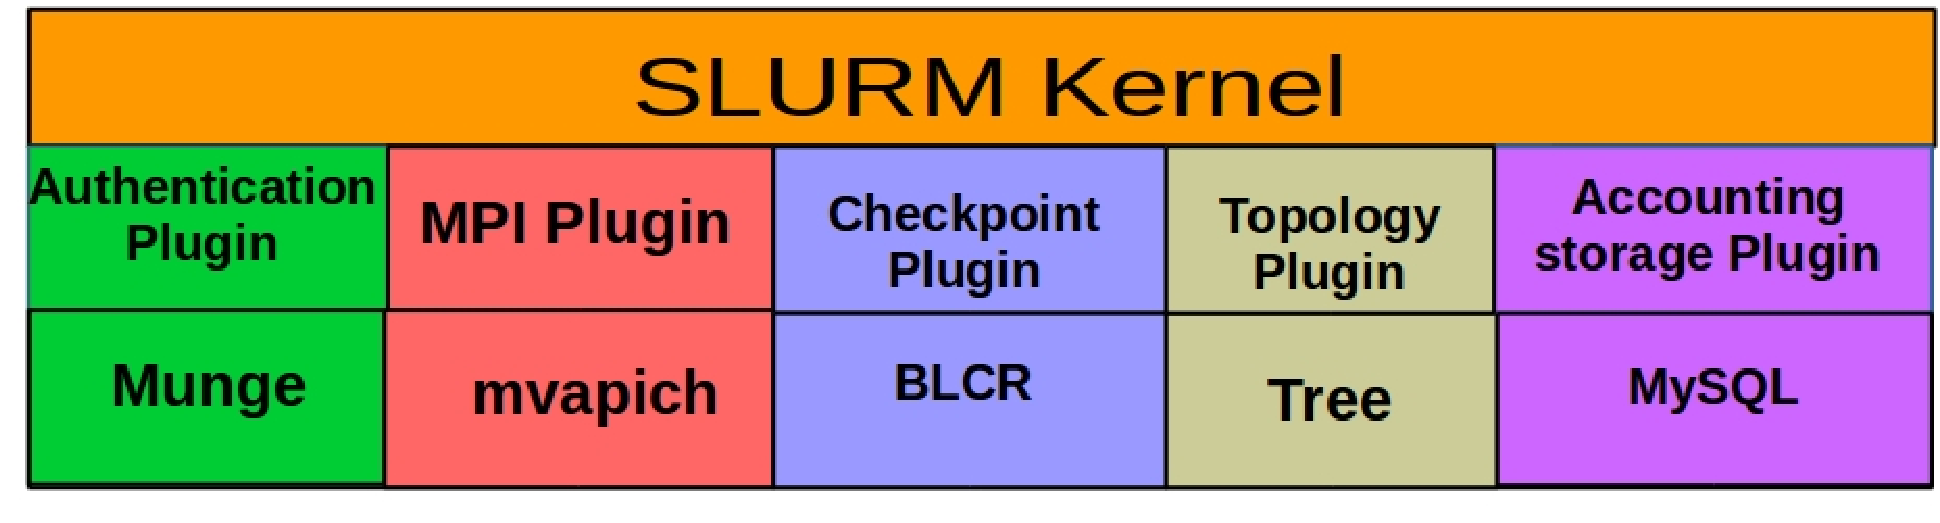
\includegraphics[width=0.43\textwidth, height=25mm]{./plugin.eps}
\caption{SLURM with optional Plugins}
\label{fig:1}
\end{figure}
\subsection{Support for Invasive Computing}
Existing batch systems usually only support static allocation of resources to applications before job start. Hence we need some kind of an Invasive Resource Management to be integrated into these existing batch systems so that we can support malleable jobs allowing us to change the allocated resources dynamically at runtime. In order to achieve we introduce the below new components:\par
\begin{itemize}
\item \textbf{\textit{Invasive Resource Manager (alias iHypervisor):}} An independent component which will talk to the batch scheduler via a protocol to obtain invasive job(s) submitted specifically to the invasic partition(A specific partition managed by iHypervisor to support invasive computing). The iHypervisor will will then perform some kind of runtime scheduling for pinning these jobs to the resources in the partition and makes these decisions in order to optimize certain local metrics such as resource utilization, power stability, energy efficiency etc. This scheduling is done at the granularity of cores and sockets. It may be possible that in the future this component will not be a separate entitiy but will be built into the batch system itself.
\item \textbf{\textit{Invasive Job Scheduler (alias iScheduler):}} This component will be a new extension built into an existing batch system for performing job scheduling. The scheduling decisions are communicated via the protocol used to speak to iHypervisor and these decisions are basically job(s) selected via a scheduling algorithm to be submitted to the iHypervisor for execution. The scheduling decisions will be made on the basis of available resources in the partition and it is the iHypervisor that communicates this to iScheduler in the form of resource offers (Real/Virtual). It can be a virtual resource offer because the iHypervisor can hide the real resources and present a rather fake view of them to iScheduler in the hope of getting a mapping of jobs to offer that is more suitable to satisfy its local metrics. Similar to iHypervisor, the iScheduler makes its decisions to optimize for certain local metrics such as high job throughput, reduced job waiting times, deadlines, priorities etc. This highlights the mismatching policies/metrics for which both the iHypervisor and iScheduler make their decisions on and hence both will be involved in some kind of a negotiation via the protocol to reach a common agreement.
\item \textbf{\textit{Negotiation Protocol:}} This protocol forms the core of the interaction between the iScheduler and iHypervisor. It allows for iHypervisor to make one or a set of resource offers to iScheduler which then needs to select jobs from its job queue to be mapped to these resource offers and finally sent back to the iHypervisor. The iHypervisor will then decide whether to accept/reject this mapping to satisfy its local metrics. If it accepts it will launch them and if it rejects then it informs this to iScheduler in addition to sending it a new resource offer. The iScheduler can also reject the resource offers in which case it will be sent a new one. On accepting an offer, the iScheduler then repeats its tasks to send back a mapping to iHypervisor and this interaction continues until both reach a common agreement. If the number of such attempts reach a threshold then both iScheduler and iHypervisor will unconditionally agree to each other closing this transaction of negotiating. After this a new transaction can start depending on whether the job queue is empty or not. If empty the iScheduler will explicitly send a request for resource offer to iHypervisor once a new job enters the queue.
\end{itemize}
\noindent
This work will implement a prototype for demonstrating how such an approach to support invasive computing with the above entities may work. It will involve implementing the iScheduler as a new plugin(multithreaded) for SLURM and iHypervisor as an Invasive Resource Manager daemon that will essentially be similar to the slurm controller daemon but will support dynamic resource management and run time scheduling. In addition, the communication mechanism between iScheduler and iHypervisor using negotiation protocol will be implemented.
\section{Design and Implementation}
This section illustrates and describes a high level design of the early prototype implemented with the help of protocol sequence diagrams and state machine diagrams. It will help to understand at a high level as to how the system has been designed to support this new approach of invasive computing and how will many of its components in the software hierarchy interact with each other with new protocols.
\subsection{Software Architecture}
Figure on the right shows the software architecture of how Invasive Resource Management can be supported with a traditional resource manager and how exactly the new software components will fit in the existing software hierarchy. This figure relates closely to how SLURM is organized since the intention of this work would be to demonstrate the support for Invasive Computing with the help of SLURM as a resource manager.
\begin{itemize}
\item The top layer is that of the core resource management component which has access to job queues. In this architecture, it will now have access to not just the queue for legacy(static) jobs but also invasic job queue(jobs submittted to invasic partition).
\item In a traditional setup the top layer will also perform Job Scheduling. This means that it will select a job(s) from the queue of jobs based on the current state of resources and other factors to dispatch it to a traditional process manager. The process manager then takes the responsibility of launching these jobs on the allocated resources in the partition and managing them for their full lifetime. 
\item The new independent component iHypervisor will now sit between the top layer and the traditional process manager to act as a virtualization layer for resources in the Invasic Partition. It will communicate with iScheduler and influence the scheduling decisions taken by it. 
\item A new plugin for SLURM by the name "iScheduler" will be implemented to handle job scheduling specifically for invasic jobs.
\item Communication between iHypervisor and iScheduler is done using the negotiation protocol. In addition iScheduler will also process periodic feedbacks sent by iHypervisor that will contain some useful statistical measures regarding current state of resources, its utilization, job throughput etc. and this may help influence the decision making of iScheduler later. 
\item Additionally there is also a dedicated communication channel to service urgent jobs immediately.
\end{itemize}
\begin{figure}[t]
\centering
\includegraphics[width=0.4\textwidth, height=90mm]{./"software architecture-eps-converted-to".pdf}
\caption{Invasive Resource Management Architecture}
\label{fig:3}
\end{figure}
\subsection{Communication Phases}
Below mentioned are the different phases one may see during the interaction between the iScheduler and iHypervisor.
\begin{itemize}
\item \textbf{\textit{Protocol Initialization:}} This phase basically establishes the initial environment between iScheduler and iHypervisor for for negotiations to start later on. Successful initialization of this phase prepares both the parties to start negotiating. During this phase various parameters such as protocl version, maximum attempts for negotiation, timer intervals and several other parameters could be exchanged to set up the internal data structures and configuration tables for both the communicating parties. This protocol is a bi-directional communication.
\item \textbf{\textit{Protocol Finalization:}} This phases signals the end of communication between iHypervisor and iScheduler using negotiation protocol. It leads to a safe termination of this communication followed by the release of any internal data structures allocated earlier along with configuration parameters. This results in consistent behaviour of both the communicating parties which can then proceed to safely terminate and exit. This protocol is a bi-directional communication.
\item \textbf{\textit{Negotiation:}} This is the most important phase where both iHypervisor and iScheduler are negotiating with each other till they reach an agreement. If they do not then they continue till a certain upper limit on the number of negotiating attempts is reached after which both of them unconditionally agree to close the current negotiation. After this a new transaction of negotiation begins.
\item \textbf{\textit{Feedback:}} This concerns the periodic feedback sent by the iHypervisor containing useful statistical measures that can influence the iScheduler in its decision making during its future negotiations. This protocol is a uni-directional communication.
\item \textbf{\textit{Urgent Jobs:}} This protocol concerns the support for urgent jobs. At any given point of time a cluster or supercomputing center may want to support very high priority jobs immediately without any delay. By introducing support for invasive computing, it makes it all the more feasible to help run these urgent jobs immediately by either shrinking the resources of other jobs or suspending/Killing them. 
\end{itemize}
The following section illustrates some sequence diagrams of how the negotiation protocol works in some of the important scenarios that will be encountered most of the time during the operation of the system. The sequence diagrams of other protocols are not shown in this paper due to space constraints and also because they are simple and commonly observed protocol types.
\subsection{Protocol Sequence Diagrams}
\begin{figure}[!htbp]
\centering
\includegraphics[width=0.4\textwidth, height=65mm]{"/home/nishanth/Thesis/Guided Research/Documentation/figures-eps-converted-to".pdf}
\caption{Scenario 1}
\label{fig:Seq1}
\end{figure}
\begin{itemize}
\item Above diagram illustrates a scenario where both iScheduler and iHpervisor are negotiating with each other. The scenario is continued in the next figure. Figure $5$ at the right illustrates another scenario where negotiations may stop when job queue becomes empty and iHypevisor will then wait for a request from iScheduler for a resource offer that will happen when new jobs arrive.
\item iScheduler makes scheduling decisions at a coarser level of granularity which is nodes whereas iHypervisor does at the granularity of cores and sockets. Both will negotiate with each other till they reach an agreement.
\item It is an event based scheduling which means iScheduler makes a scheduling decision only when it is triggered by receiving a resource offer from iHypervisor. It is only at the start when there are no jobs in the queue and during the operations when the queue may become empty that the iScheduler will have to explicitly send a request message to iHypervisor for a resource offer otherwise at all other times scheduling is event based.
\end{itemize}
\begin{figure}[t]
\centering
\includegraphics[width=0.4\textwidth, height=50mm]{"/home/nishanth/Thesis/Guided Research/Documentation/figures1-eps-converted-to".pdf}
\caption{Scenario 1 contd.}
\label{fig:Seq2}
\end{figure}
\begin{figure}[!htbp]
\centering
\includegraphics[width=0.4\textwidth, height=50mm]{"/home/nishanth/Thesis/Guided Research/Documentation/figures2-eps-converted-to".pdf}
\caption{Scenario 2}
\label{fig:Seq3}
\end{figure}
%\section{State Machine Diagram}
%Figure \ref{fig:iScheduler} on the next page illustrates at a high level the state machine diagram of the iScheduler and how it handles the resource offers and scheduling(currently being implemented).
\begin{figure}[t]
\includegraphics[width=0.47\textwidth, height=100mm]{"/home/nishanth/Thesis/Guided Research/Documentation/Negotiation-eps-converted-to".pdf}
\caption{Flow Chart for iScheduler}
\label{fig:iScheduler}
\end{figure}
\section{State Machine Diagram}
Figure \ref{fig:iScheduler} on the next page illustrates at a high level the state machine diagram of the iScheduler and how it handles the resource offers and scheduling(currently being implemented).
\section{Related Work}
\section{Conclusions}
The objective of this research work was to implement an early prototype with the protocols proposed above and a bare minimum implementation of the new components in the architecture. This serves as a basic groundwork for the ongoing research work that in the coming months will propose and develop concrete implementations of scheduling algorithms, run time tuning of parallel applications, optimizing decision making at both the levels of iScheduler and iHypervisor through different approaches one of which could be machine learning. The basic communication infrastructure including the skeleton of protocol messages and the respective multithreaded communicating parties have been successfully implemented and tested for correctness.
%\end{document}  % This is where a 'short' article might terminate

% The following two commands are all you need in the
% initial runs of your .tex file to
% produce the bibliography for the citations in your paper.
\bibliographystyle{abbrv}
\bibliography{sigproc}  % sigproc.bib is the name of the Bibliography in this case
\nocite{felix,laxmikant,nikolas,rudolph,isaias,andreas,georgiou,travis,gladys,klein,pavan,jette,slurm}
% You must have a proper ".bib" file
%  and remember to run:
% latex bibtex latex latex
% to resolve all references
%
% ACM needs 'a single self-contained file'!
%
\balancecolumns
% That's all folks!
\end{document}
